\documentclass[aspectratio=169,11pt]{beamer}

% Theme
\usetheme{Madrid}
\usecolortheme{seahorse}

% Packages
\usepackage[utf8]{inputenc}
\usepackage[T1]{fontenc}
\usepackage[brazilian]{babel}
\usepackage{graphicx}
\usepackage{booktabs}
\usepackage{tikz}
\usepackage{xcolor}
\usepackage{fontawesome5}

% Custom colors
\definecolor{revoBlue}{RGB}{52, 152, 219}
\definecolor{revoRed}{RGB}{231, 76, 60}
\definecolor{revoGreen}{RGB}{39, 174, 96}
\definecolor{revoDark}{RGB}{44, 62, 80}
\definecolor{revoOrange}{RGB}{230, 126, 34}

\setbeamercolor{frametitle}{bg=revoDark,fg=white}
\setbeamercolor{title}{bg=revoDark,fg=white}
\setbeamercolor{structure}{fg=revoBlue}
\setbeamercolor{block title}{bg=revoBlue,fg=white}
\setbeamercolor{block body}{bg=revoBlue!10}

% Title
\title[\textbf{Analise Helicoptero vs Carro}]{\textbf{Analise de Tempo de Viagem:\\Helicoptero vs Carro}}
\subtitle{Uma Comparacao Abrangente de Cenarios de Trafego\\Nova York \& Los Angeles}
\author{REVO Helicopter Services}
\institute{Divisao de Analise Estrategica}
\date{Dezembro 2025}

% Logo
\logo{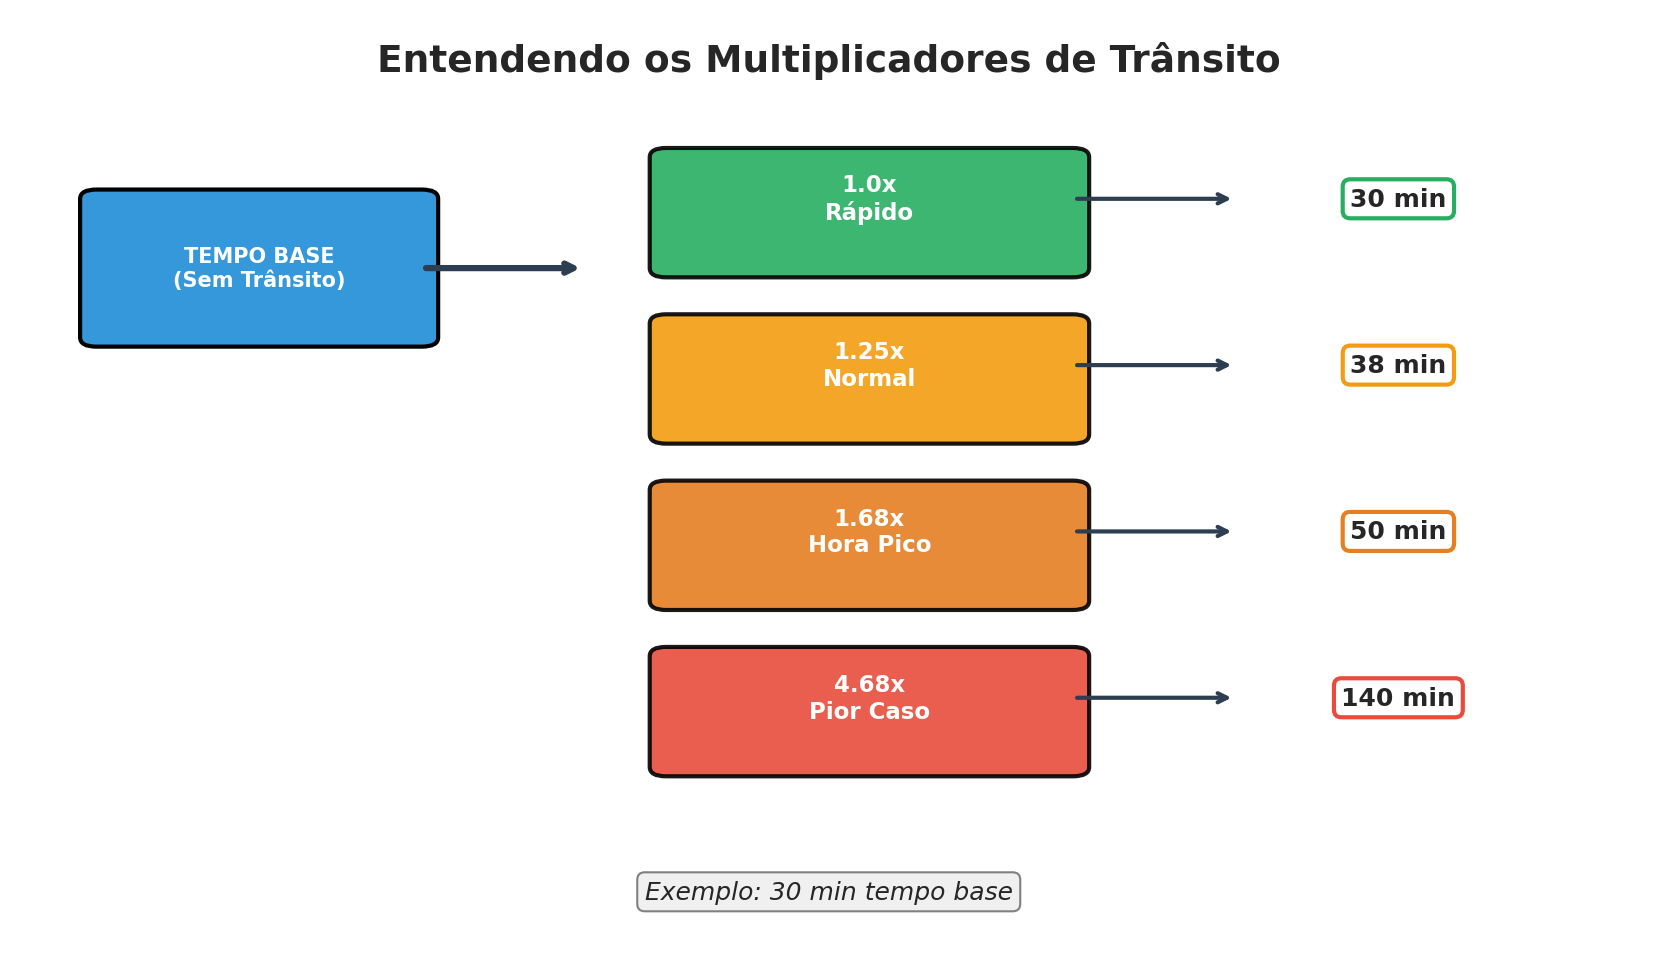
\includegraphics[height=0.8cm]{../diagrams/traffic_multiplier_pt.png}}

\begin{document}

% ============================================================================
% TITLE SLIDE
% ============================================================================
\begin{frame}
\titlepage
\end{frame}

% ============================================================================
% AGENDA
% ============================================================================
\begin{frame}{Agenda}
\tableofcontents
\end{frame}

% ============================================================================
\section{Introducao}
% ============================================================================

\begin{frame}{O Problema: Congestionamento do Trafego Urbano}
\begin{columns}
\column{0.5\textwidth}
\begin{block}{O Desafio}
\begin{itemize}
    \item Viajantes de negocios precisam de acesso confiavel ao aeroporto
    \item Trafego e imprevisivel e frequentemente severo
    \item Perder voos = impacto significativo nos negocios
    \item Estresse e perda de tempo afetam produtividade
\end{itemize}
\end{block}

\column{0.5\textwidth}
\begin{alertblock}{Realidade do Pior Caso}
\begin{center}
\textbf{Durante trafego severo:}\\[0.5em]
\Large{\textcolor{revoRed}{4.68x}} \normalsize{tempo de viagem}\\[0.5em]
\Large{\textcolor{revoRed}{12 km/h}} \normalsize{velocidade media}\\[0.5em]
\textit{(mal mais rapido que caminhar!)}
\end{center}
\end{alertblock}
\end{columns}
\end{frame}

\begin{frame}{Visao Geral do Estudo}
\begin{columns}
\column{0.6\textwidth}
\begin{block}{Escopo}
\begin{itemize}
    \item \textbf{Nova York}: 70 CEPs de alta renda $\rightarrow$ JFK
    \item \textbf{Los Angeles}: 44 CEPs de alta renda $\rightarrow$ LAX
    \item \textbf{Dados}: Google Traffic (Pessimista)
    \item \textbf{Roteamento}: OSRM + Dados FAA de Helipontos
\end{itemize}
\end{block}

\column{0.4\textwidth}
\begin{exampleblock}{Numeros Chave}
\begin{center}
\Large{114} \normalsize{CEPs}\\[0.3em]
\Large{65} \normalsize{Heliportos}\\[0.3em]
\Large{4} \normalsize{Cenarios de Trafego}\\[0.3em]
\Large{27} \normalsize{CEPs Manhattan}
\end{center}
\end{exampleblock}
\end{columns}
\end{frame}

% ============================================================================
\section{Metodologia}
% ============================================================================

\begin{frame}{Multiplicadores de Trafego Explicados}
\begin{center}
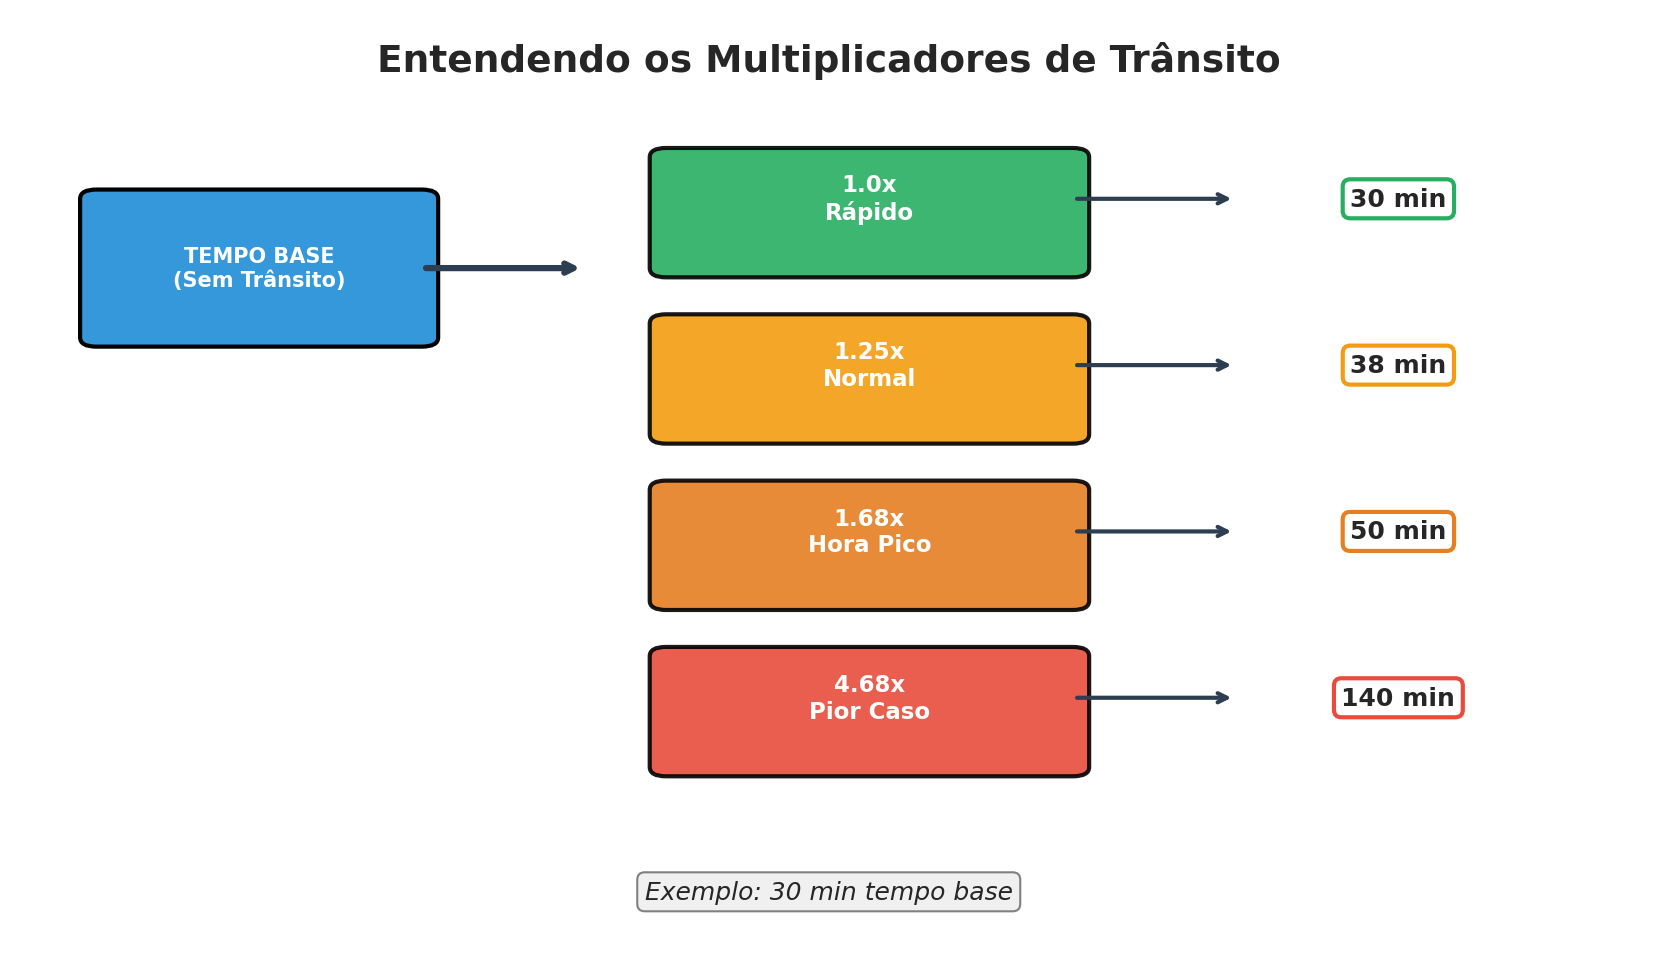
\includegraphics[width=0.75\textwidth]{../diagrams/traffic_multiplier_pt.png}
\end{center}
\end{frame}

\begin{frame}{Comparacao de Trajeto: Carro vs Helicoptero}
\begin{center}
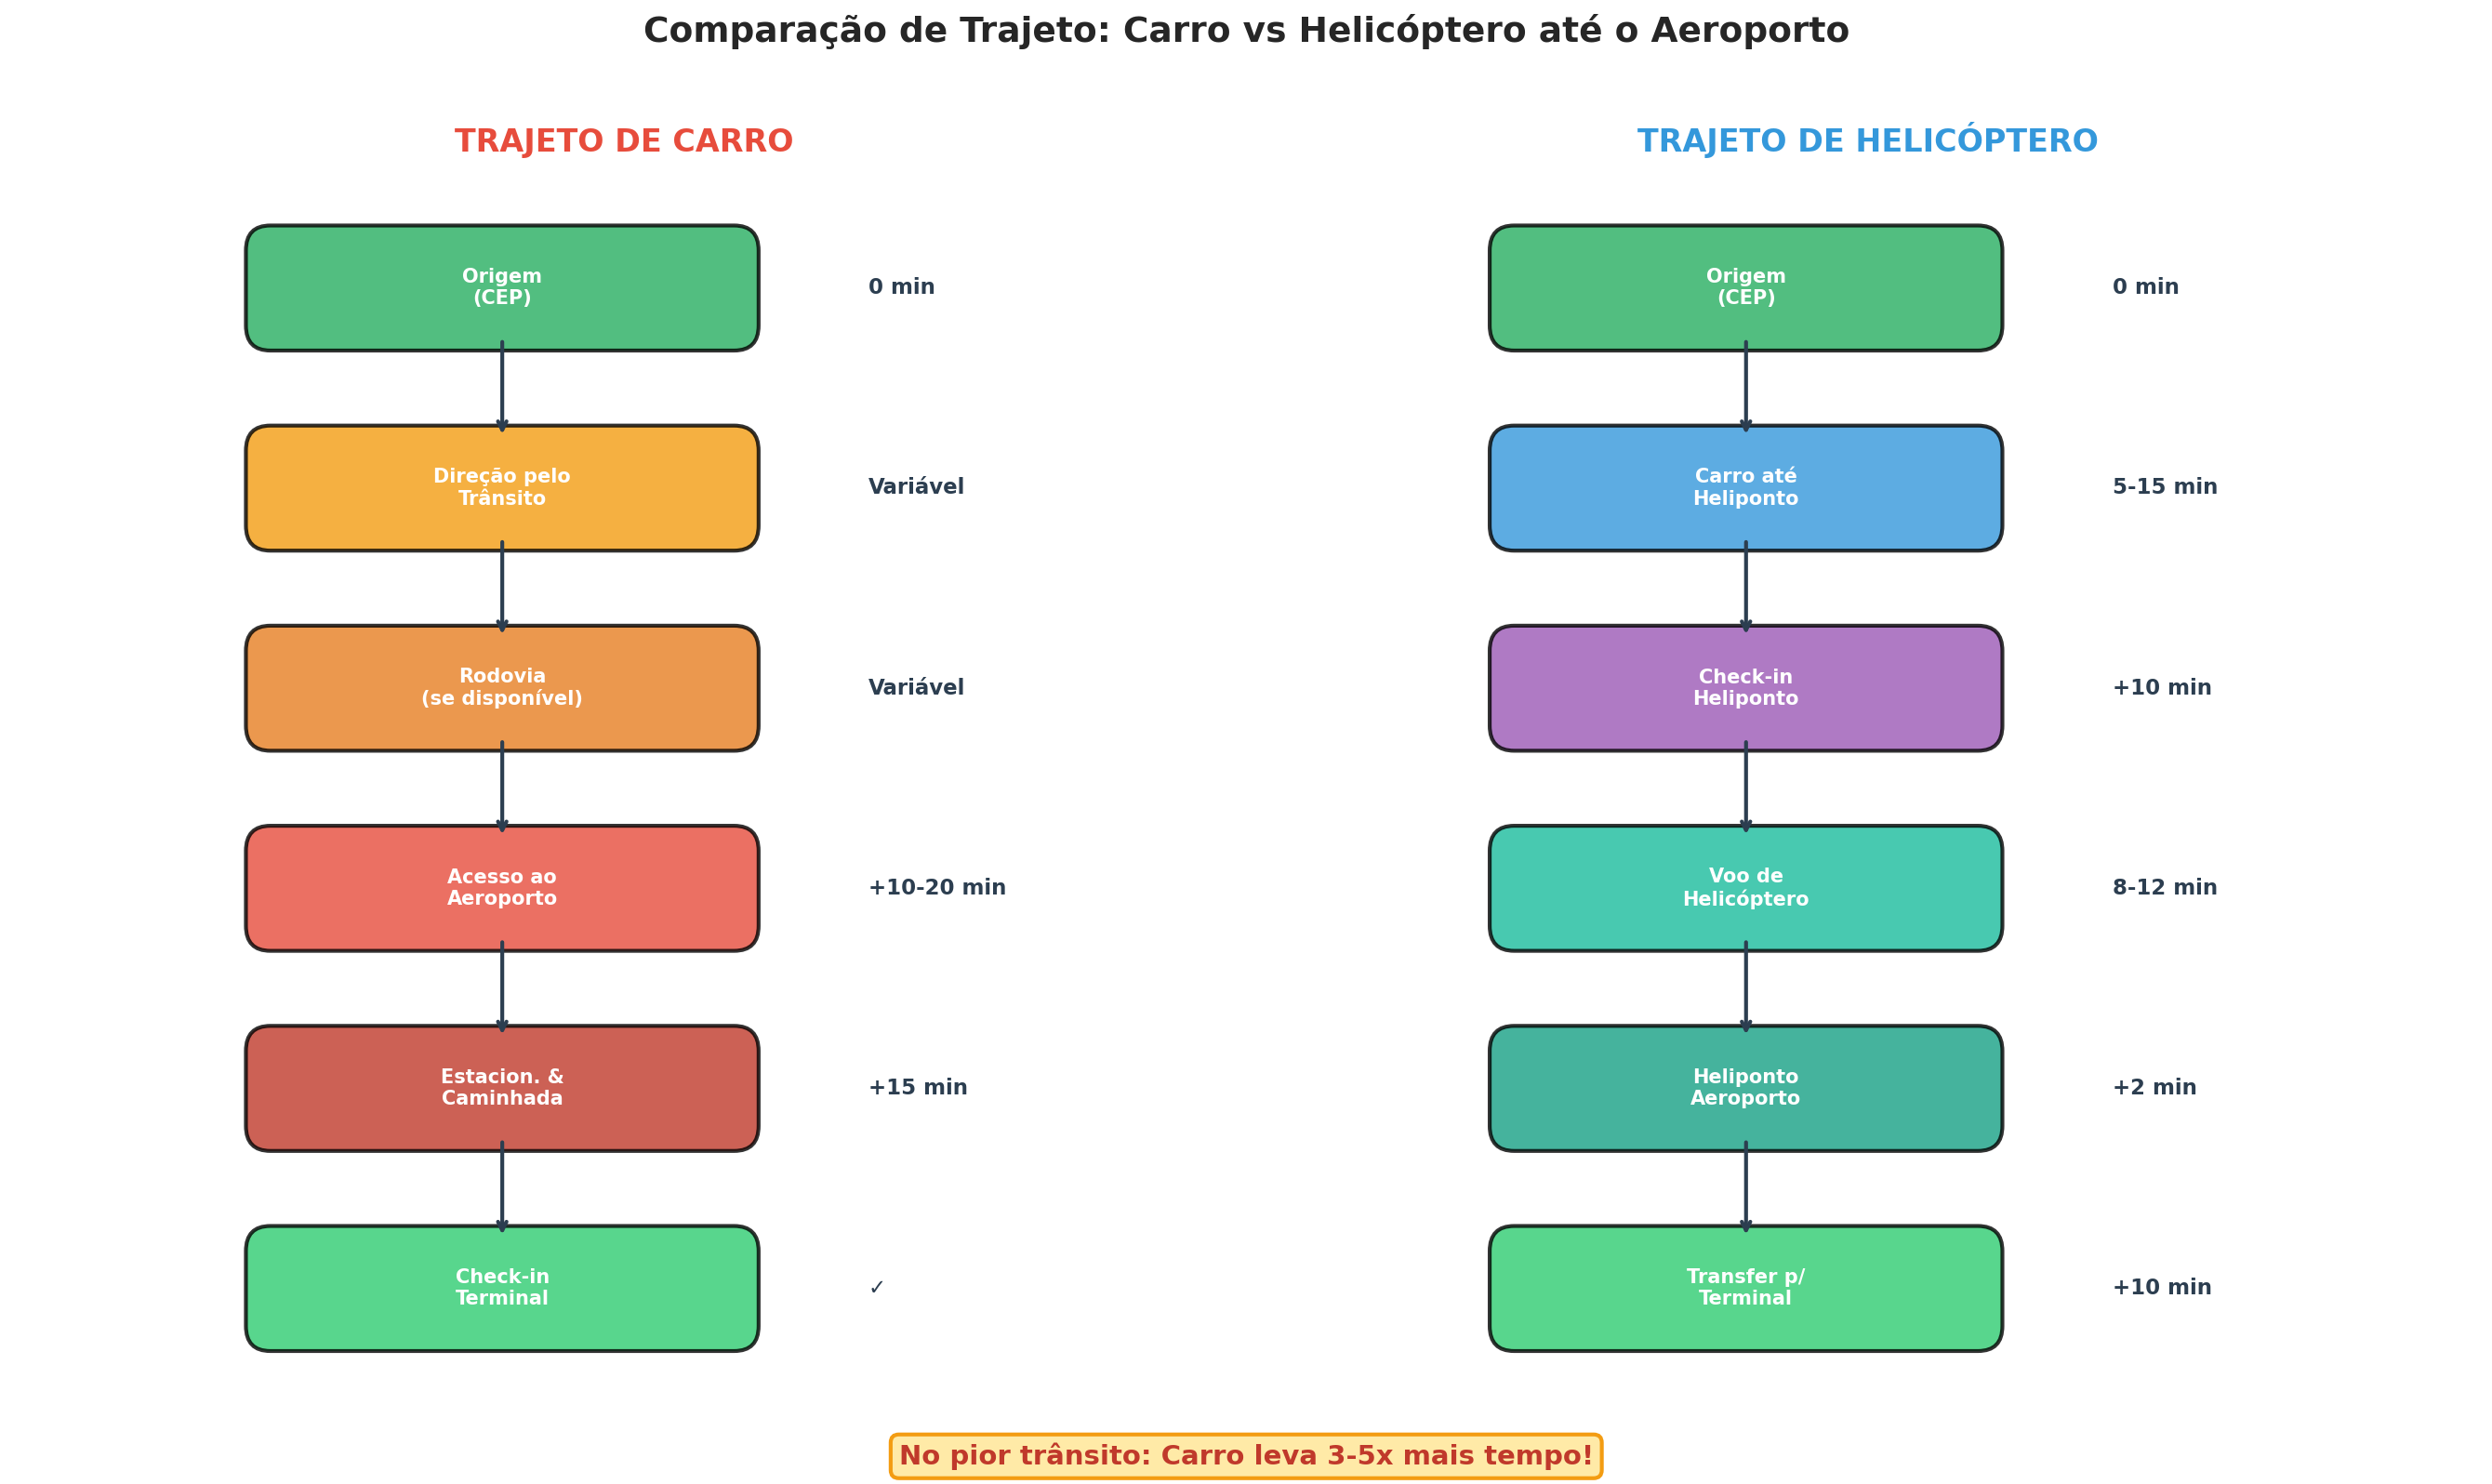
\includegraphics[width=0.95\textwidth]{../diagrams/journey_diagram_pt.png}
\end{center}
\end{frame}

\begin{frame}{Componentes do Trajeto de Helicoptero}
\begin{columns}
\column{0.5\textwidth}
\begin{block}{\faCarSide\ Etapa 1: Carro ate Heliponto}
\begin{itemize}
    \item Afetado pelo trafego
    \item Prioridade para heliponto em Manhattan
    \item Media: 5-15 minutos
\end{itemize}
\end{block}

\begin{block}{\faHelicopter\ Etapa 3: Voo}
\begin{itemize}
    \item Velocidade de cruzeiro 200 km/h
    \item Rota direta
    \item 8-12 minutos tipico
\end{itemize}
\end{block}

\column{0.5\textwidth}
\begin{block}{\faClipboardCheck\ Etapa 2: Check-in}
\begin{itemize}
    \item 10 minutos fixos
    \item Triagem de seguranca
    \item Preparacao para embarque
\end{itemize}
\end{block}

\begin{block}{\faWalking\ Etapa 4: Transfer para Terminal}
\begin{itemize}
    \item 10 minutos fixos
    \item Heliponto ao terminal
    \item Transporte interno
\end{itemize}
\end{block}
\end{columns}
\end{frame}

\begin{frame}{Rede de Helipontos de Manhattan}
\begin{columns}
\column{0.5\textwidth}
\begin{block}{Heliportos Aprovados}
\begin{itemize}
    \item \textbf{JRB}: Downtown/Wall St
    \item \textbf{JRA}: West 30th Street
    \item \textbf{6N5}: East 34th Street
    \item \textbf{3NY2}: Astoria (Queens)
\end{itemize}
\end{block}

\begin{alertblock}{Exclusoes}
\faTimesCircle\ Heliportos de Policia\\
\faTimesCircle\ One Police Plaza\\
\faTimesCircle\ Newport Beach Police (LA)
\end{alertblock}

\column{0.5\textwidth}
\begin{center}
\textbf{Por que Apenas Manhattan?}\\[1em]
\begin{tikzpicture}[scale=0.8]
    \draw[thick, fill=revoBlue!20] (0,0) rectangle (2,4);
    \node at (1,3.5) {\small Manhattan};
    \draw[ultra thick, revoRed] (2,2) -- (4,2);
    \node[revoRed] at (3,2.5) {\small \faTimesCircle\ Pontes};
    \node[revoRed] at (3,1.5) {\small \faTimesCircle\ Tuneis};
    \draw[thick, fill=gray!20] (4,0) rectangle (6,4);
    \node at (5,2) {\small NJ/Queens};
\end{tikzpicture}\\[1em]
\textit{Evitar travessias congestionadas!}
\end{center}
\end{columns}
\end{frame}

% ============================================================================
\section{Resultados}
% ============================================================================

\begin{frame}{Visao Geral da Comparacao de Cenarios}
\begin{center}

\includegraphics[width=0.95\textwidth]{../comparison_charts_pt/fig1_scenario_comparison.png}
\end{center}
\end{frame}

\begin{frame}{Estatisticas Principais}
\begin{table}
\centering
\begin{tabular}{l|cccc|cccc}
\toprule
& \multicolumn{4}{c|}{\textcolor{revoBlue}{\textbf{Nova York}}} & \multicolumn{4}{c}{\textcolor{revoRed}{\textbf{Los Angeles}}} \\
\textbf{Metrica} & Rap & Norm & Pico & Pior & Rap & Norm & Pico & Pior \\
\midrule
Carro (min) & 47 & 59 & 79 & \textbf{221} & 47 & 59 & 80 & \textbf{222} \\
Heli (min) & 44 & 46 & 49 & \textbf{74} & 46 & 48 & 52 & \textbf{79} \\
\rowcolor{revoGreen!30} Economia & 3 & 13 & 30 & \textbf{147} & 1 & 11 & 28 & \textbf{143} \\
\bottomrule
\end{tabular}
\end{table}

\begin{center}
\Large{\textcolor{revoGreen}{\textbf{Pior Caso: Economize 2+ Horas!}}}
\end{center}
\end{frame}

\begin{frame}{Degradacao de Velocidade por Cenario}
\begin{center}

\includegraphics[width=0.9\textwidth]{../comparison_charts_pt/fig2_speed_comparison.png}
\end{center}
\end{frame}

\begin{frame}{Distribuicao de Economia de Tempo}
\begin{center}

\includegraphics[width=0.95\textwidth]{../comparison_charts_pt/fig4_savings_boxplot.png}
\end{center}
\end{frame}

\begin{frame}{Normal vs Pior Caso: A Diferenca Dramatica}
\begin{center}

\includegraphics[width=0.9\textwidth]{../comparison_charts_pt/fig6_normal_vs_worst.png}
\end{center}
\end{frame}

\begin{frame}{Como o Trafego Multiplica o Tempo de Viagem}
\begin{center}

\includegraphics[width=0.9\textwidth]{../comparison_charts_pt/fig5_multiplier_effect.png}
\end{center}
\end{frame}

\begin{frame}{Tempo por 100 Metros}
\begin{center}

\includegraphics[width=0.9\textwidth]{../comparison_charts_pt/fig3_time_100m.png}
\end{center}

\begin{columns}
\column{0.5\textwidth}
\begin{center}
\textbf{Pior Caso:}\\
30 segundos / 100m
\end{center}

\column{0.5\textwidth}
\begin{center}
\textbf{Caminhando:}\\
72 segundos / 100m
\end{center}
\end{columns}
\end{frame}

\begin{frame}{Detalhamento do Tempo: Pior Caso}
\begin{center}
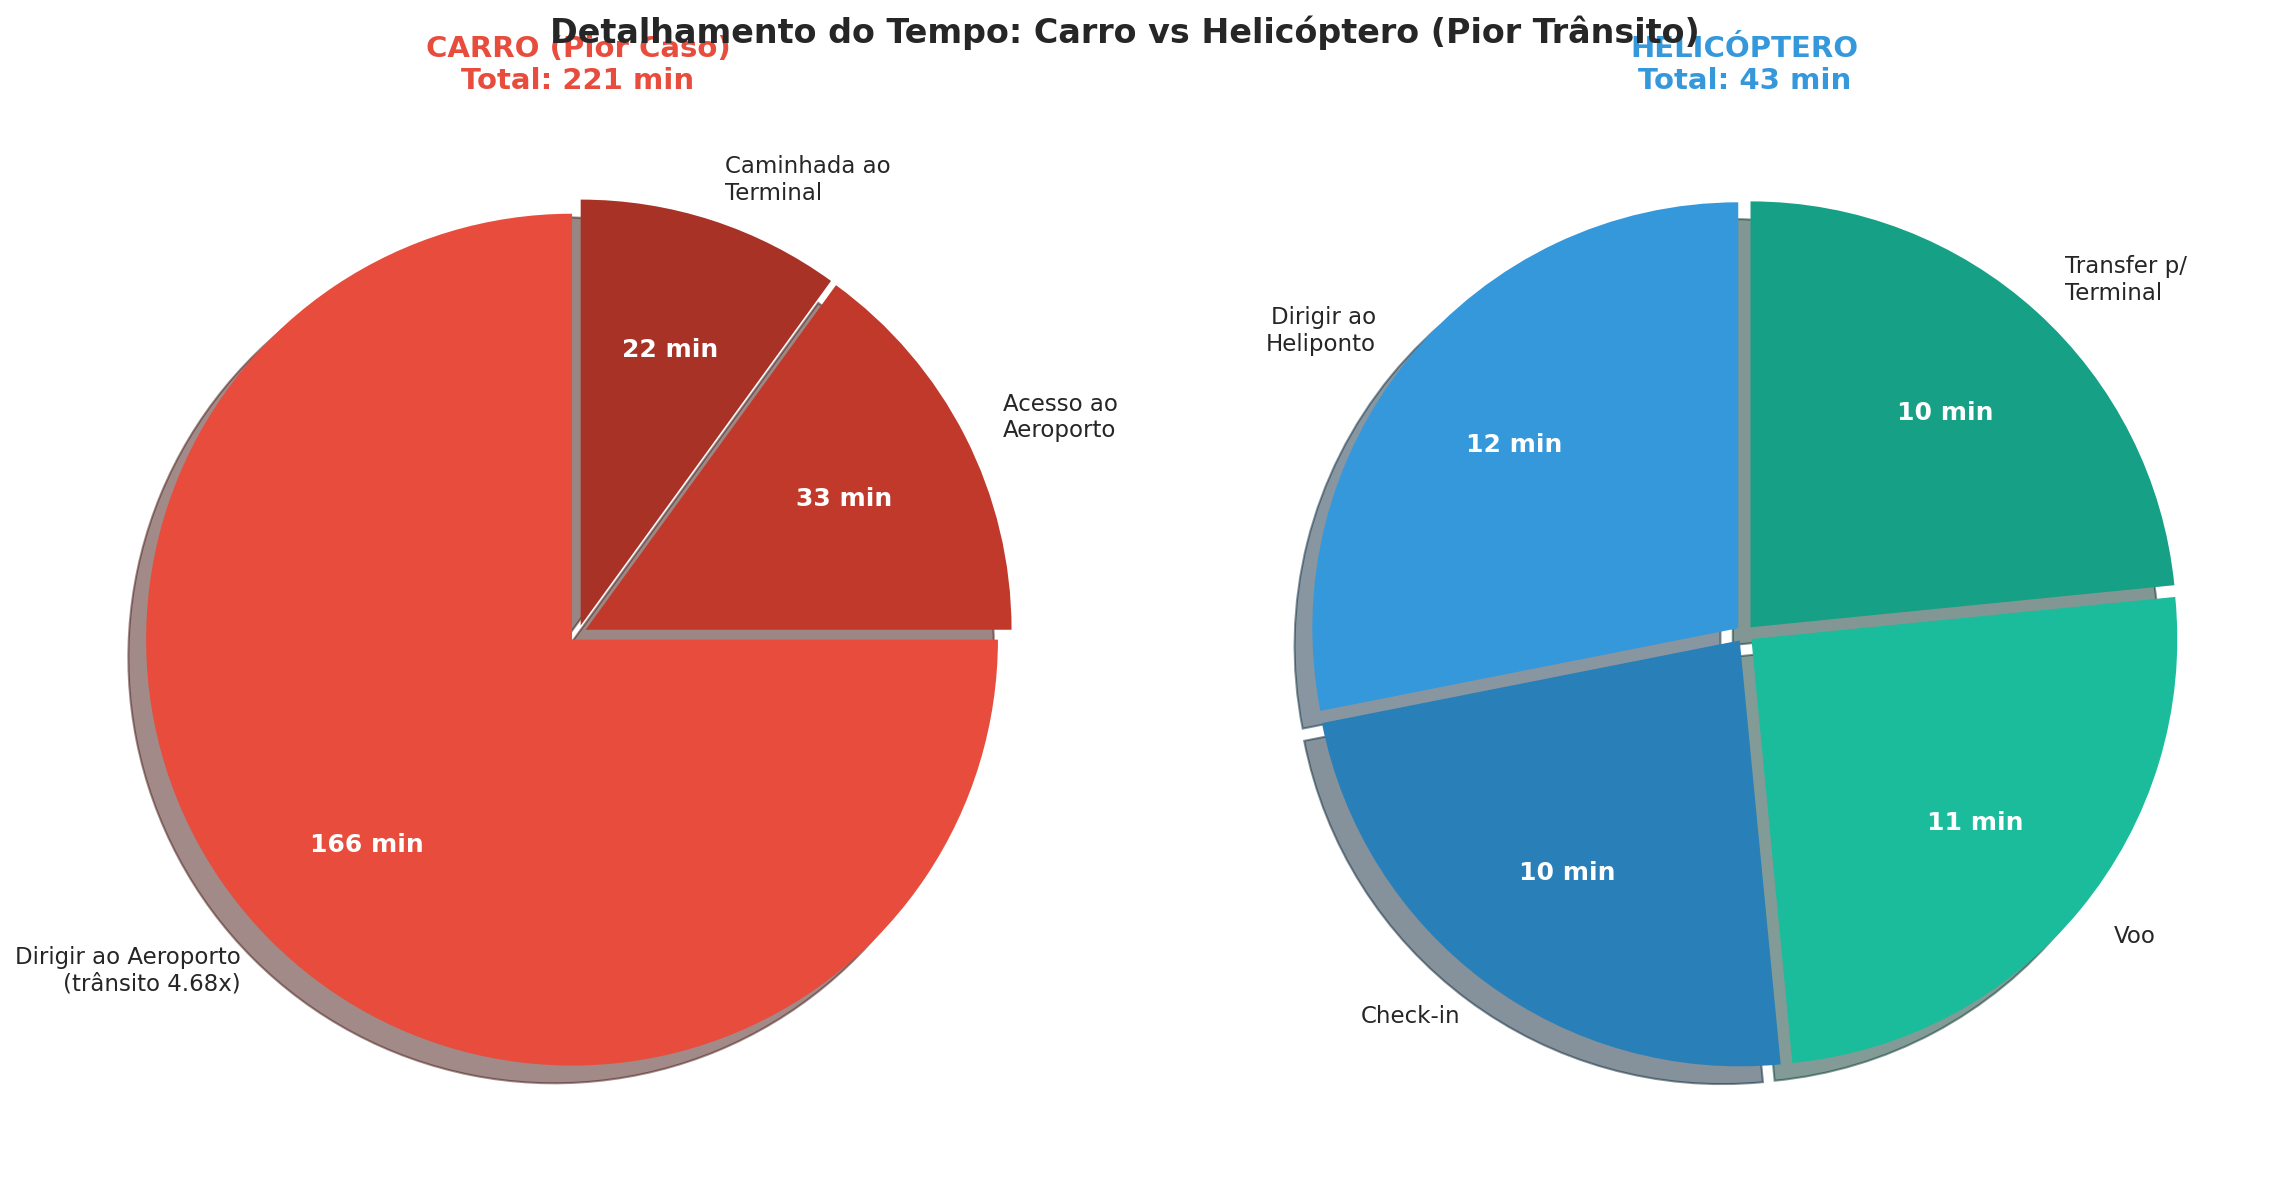
\includegraphics[width=0.8\textwidth]{../diagrams/time_breakdown_pt.png}
\end{center}
\end{frame}

\begin{frame}{Histograma de Distribuicao de Economia}
\begin{center}

\includegraphics[width=0.95\textwidth]{../comparison_charts_pt/fig8_savings_histogram.png}
\end{center}
\end{frame}

% ============================================================================
\section{Insights Principais}
% ============================================================================

\begin{frame}{Por que o Helicoptero Vence no Pior Caso}
\begin{columns}
\column{0.5\textwidth}
\begin{block}{\faCarSide\ Viagem de Carro}
\begin{itemize}
    \item \textcolor{revoRed}{\textbf{100\%}} afetado pelo trafego
    \item Tempo aumenta \textcolor{revoRed}{\textbf{4.68x}}
    \item Atrasos imprevisiveis
    \item Estresse e fadiga
\end{itemize}
\end{block}

\column{0.5\textwidth}
\begin{block}{\faHelicopter\ Viagem de Helicoptero}
\begin{itemize}
    \item Apenas \textcolor{revoGreen}{\textbf{20\%}} afetado pelo trafego
    \item Tempo aumenta apenas \textcolor{revoGreen}{\textbf{1.6x}}
    \item Agenda previsivel
    \item Conforto e produtividade
\end{itemize}
\end{block}
\end{columns}

\vspace{1em}
\begin{center}
\begin{tikzpicture}
    \draw[ultra thick, ->, revoBlue] (0,0) -- (10,0);
    \node at (5,-0.5) {Severidade do Trafego};
    \draw[thick, revoRed] (0,0.5) -- (10,3);
    \node[revoRed] at (10.5,3) {Carro};
    \draw[thick, revoGreen] (0,0.5) -- (10,1);
    \node[revoGreen] at (10.5,1) {Heli};
\end{tikzpicture}
\end{center}
\end{frame}

\begin{frame}{Proposta de Valor para Negocios}
\begin{columns}
\column{0.33\textwidth}
\begin{center}
\textcolor{revoBlue}{\Huge{\faClock}}\\[0.5em]
\textbf{Economia de Tempo}\\[0.5em]
\Large{147 min}\\
\normalsize{(NY pior caso)}
\end{center}

\column{0.33\textwidth}
\begin{center}
\textcolor{revoGreen}{\Huge{\faCheckCircle}}\\[0.5em]
\textbf{Confiabilidade}\\[0.5em]
\Large{99\%}\\
\normalsize{taxa de vantagem}
\end{center}

\column{0.33\textwidth}
\begin{center}
\textcolor{revoOrange}{\Huge{\faPlane}}\\[0.5em]
\textbf{Nunca Perca}\\[0.5em]
\Large{Voos}\\
\normalsize{chegada previsivel}
\end{center}
\end{columns}

\vspace{1em}
\begin{exampleblock}{Consideracao de ROI}
2+ horas economizadas = tempo produtivo para reunioes, menos estresse, conexoes garantidas
\end{exampleblock}
\end{frame}

% ============================================================================
\section{Conclusoes}
% ============================================================================

\begin{frame}{Resumo das Descobertas}
\begin{columns}
\column{0.5\textwidth}
\begin{block}{\textcolor{revoBlue}{Nova York}}
\begin{itemize}
    \item 70 CEPs analisados
    \item 27 locais em Manhattan
    \item \textbf{147 min} economia pior caso
    \item \textbf{66\%} reducao de tempo
    \item 99\% mostram vantagem do helicoptero
\end{itemize}
\end{block}

\column{0.5\textwidth}
\begin{block}{\textcolor{revoRed}{Los Angeles}}
\begin{itemize}
    \item 44 CEPs analisados
    \item Cobertura distribuida
    \item \textbf{143 min} economia pior caso
    \item \textbf{64\%} reducao de tempo
    \item 98\% mostram vantagem do helicoptero
\end{itemize}
\end{block}
\end{columns}

\vspace{1em}
\begin{alertblock}{Conclusao Principal}
\centering
Quanto pior o trafego, maior a vantagem do helicoptero.\\
Em condicoes extremas, o helicoptero e a \textbf{unica opcao viavel} para viagens sensiveis ao tempo.
\end{alertblock}
\end{frame}

\begin{frame}{Estatisticas Resumidas Completas}
\begin{center}

\includegraphics[width=0.95\textwidth]{../comparison_charts_pt/fig7_summary_table.png}
\end{center}
\end{frame}

\begin{frame}
\begin{center}
\Huge{\textbf{Obrigado}}\\[2em]
\Large{Perguntas?}\\[2em]
\normalsize{REVO Helicopter Services}\\
\textit{Divisao de Analise Estrategica}\\[1em]
Dezembro 2025
\end{center}
\end{frame}

\end{document}

